\documentclass{beamer}
%\documentclass[notes]{beamer} %Use this instead of the first line for displaying the notes
\usetheme{Berlin}
\usepackage{amsmath}
\usepackage{amsthm}
\usepackage{blindtext}
\usepackage{amsfonts}
\usepackage{graphicx}
\usepackage{tabto}
\usepackage{csquotes}

\title{Representation theory of finite groups}
\subtitle{Formalization project}
\author{Raphael Gaedtke, Paul Neumann}
\institute{University of Bonn}
\date{January 10, 2025}

\newcommand{\GL}{\text{GL}}
\newcommand{\Img}{\text{Im}}
\newcommand{\Ker}{\text{Ker}}
\newcommand{\inv}{^{-1}}
\newcommand{\R}{\mathbb{R}}

\begin{document}
\begin{frame}
\titlepage
\end{frame}

\begin{frame}
\frametitle{Outline}
\tableofcontents
\end{frame}

\section{Representation Theory}
\begin{frame}
\frametitle{Representations of finite groups}
\begin{definition}
For a group \(G\) and a field \(k\), a \textbf{representation} of \(G\) over \(k\) is a pair \((V, \rho)\) where \(V\) is a vector space over \(k\) and \(\rho: G\to \GL (V)\) is an action of \(G\) on \(V\).
\end{definition}
\pause
Convention: \(V\) has finite dimension, unless explicitly stated otherwise.
\begin{definition}
\(\dim (V)\) is the \textbf{dimension} or \textbf{degree} of \((V, \rho)\).
\end{definition}
\end{frame}

\note{
\begin{itemize}
\item intuition of a symmetry group
\item this definition is somewhat restricted: Monoid instead of group, module instead of vector space is possible
\item Representation theory is not restricted to groups, this is a special case
\end{itemize}
}

\begin{frame}
\begin{example}
\begin{equation*}
D_{2n} = \langle a, b \vert a^n = b^2 = 1, bab = a\inv \rangle
\end{equation*}
\begin{figure}[h]
\begin{center}
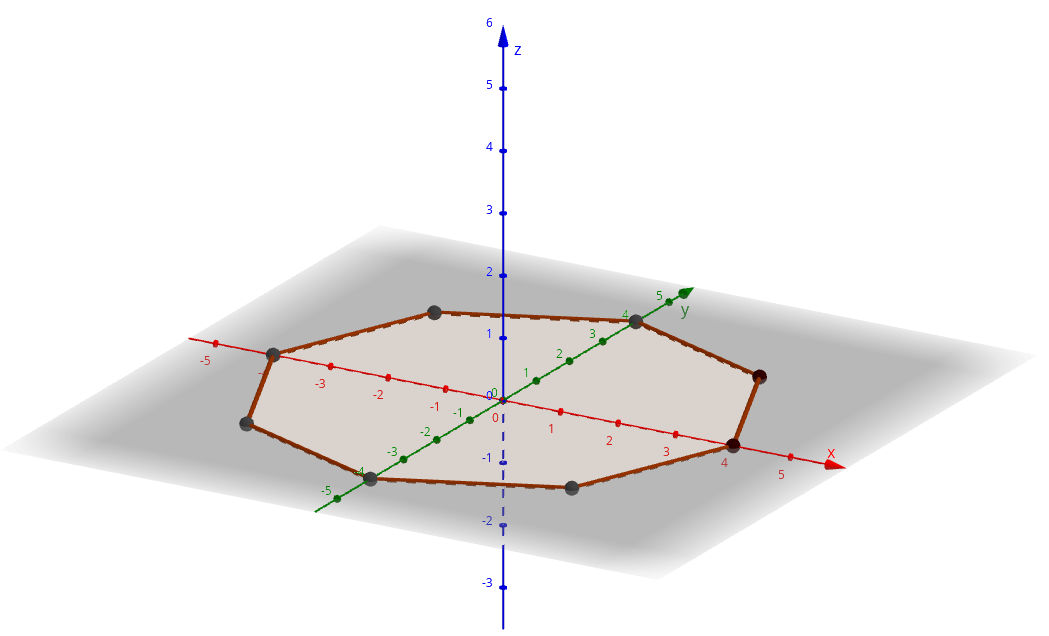
\includegraphics[width = 5cm]{images/octagon.png}
\end{center}
\end{figure}
\pause
Representation \(\rho: D_{2n} \to \GL (\R^3)\) with 
\begin{itemize}
\item \(\rho(a)\) as rotation about the \(Z\)-axis
\item \(\rho(b)\) as a rotation about a suitable axis in the \(XY\)-plane
\end{itemize}
\end{example}
\end{frame}

\begin{frame}
\frametitle{Invariant subspaces, Irreducibility}
\begin{definition}
Let \(V\) be a representation and \(U \subseteq V\) a subspace. \(U\) is an \textbf{invariant subspace} if \(gu \in U\) for \(\forall u\in U, g \in G\).
\end{definition}
\pause
\begin{example}
\begin{figure}[h]
\begin{center}
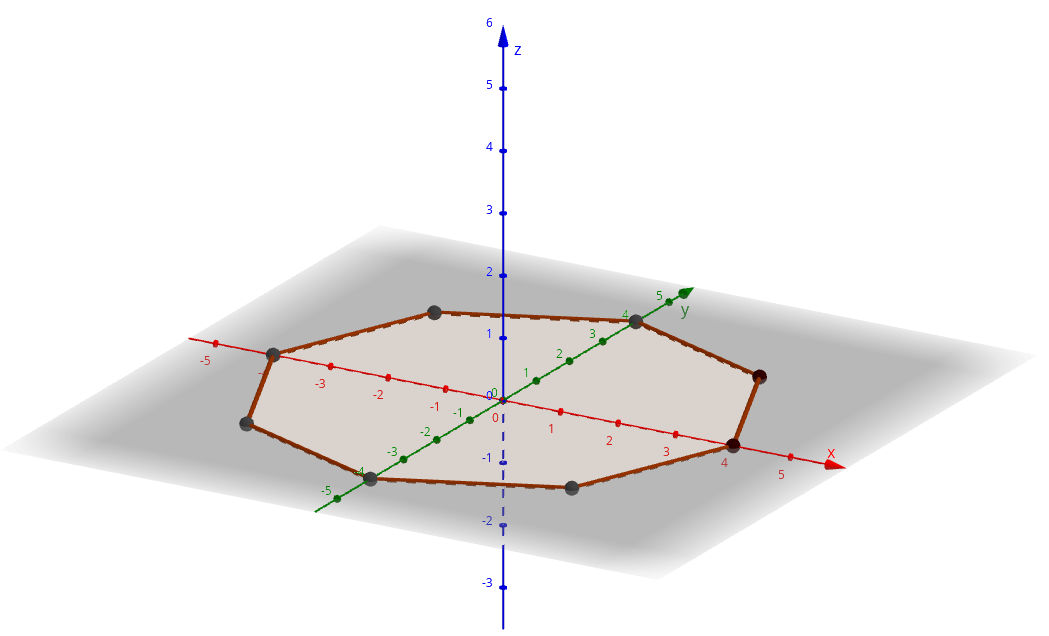
\includegraphics[width = 3cm]{images/octagon.png}
\end{center}
\end{figure}
\pause
The \(XY\)-Plane is an invariant subspace.
\end{example}
\end{frame}

\begin{frame}
\frametitle{Irreducibility, Representation Homomorphisms}
\begin{definition}
A representation \(V\) is \textbf{irreducible} provided \(V \neq 0\) and the only invariant subspaces are 0 and \(V\).
\end{definition}
\pause
\begin{definition}
For representations \(V\) and \(W\), a \textbf{homomorphism} is a linear map \(\theta: V\to W\) with \(\theta(gv) = g\theta(v)\) for \(\forall g\in G, v\in V\).
\end{definition}
\pause
\begin{itemize}
\item \(\Img (\theta)\) and \(\Ker (\theta)\) are invariant subspaces
\item If \(V\) and \(W\) are irreducible, then \(\theta: V \to W\) is 0 or bijective.
\end{itemize}
\end{frame}

\section{Finite abelian groups}
\begin{frame}
\frametitle{Main theorem formalized in this project}
This theorem is listed on the \enquote{Missing undergraduate mathematics in mathlib}-page.
\pause
\begin{theorem}
Let \(G\) be a finite abelian group.\\
Let \(V\) be a non-null vector space over an algebraically closed field \(k\).\\
Let \(\rho: G \to \GL (V)\) be a representation.\\
\pause
\vspace{1cm}
Then \(\rho\) is irreducible if and only if \(\dim_k(V) = 1\).
\end{theorem}
\end{frame}

\begin{frame}
\frametitle{Proof of the theorem}
\begin{theorem}
\(\rho\) is irreducible if and only if \(\dim_k(V) = 1\).
\end{theorem}
\enquote{\(\Leftarrow\)} is trivial.\\
For \enquote{\(\Rightarrow\)}, we use the following two lemmas:
\begin{lemma}
For all \(g \in G\), \(\rho(g)\) is a Representation Endomorphism.
\end{lemma}
\begin{lemma}
Every Representation Endomorphism is given by multiplication with a scalar.
\end{lemma}
\end{frame}

\note{
\begin{itemize}
\item in the first lemma, we use the fact that \(G\) is abelian
\item the second lemma is a corollary of Schur's lemma
\end{itemize}
}

\begin{frame}
\frametitle{Proof of the theorem}
With these two lemmas, we can prove the following fact:
\begin{lemma}
Every one-dimensional subspace of \(V\) is an invariant subspace.
\end{lemma}
\pause
Now, we can use proof by contradiction:
\pause
\begin{enumerate}
\item Assume \(\dim (V) > 1\).
\pause
\item Then, \(V\) has a proper subspace with dimension 1.
\pause
\item So \(V\) has a proper invariant subspace.
\pause
\item This is a contradiction to the irreducibility of \(V\).
\end{enumerate}
\end{frame}

\section{Formalization}
\begin{frame}
\end{frame}

\section{Mathlib}
\begin{frame}
\end{frame}

\section{Future work}
\begin{frame}
\end{frame}

\end{document}